\documentclass{sig-alternate-05-2015}

\usepackage{xcolor}
\usepackage{pifont}
\usepackage{paralist} % inparaenum support

\newcommand{\quadrat}{\ding{110}}%


\begin{document}
% No indent of paragraph
\parindent 0pt

% Copyright
\setcopyright{acmcopyright}
%\setcopyright{acmlicensed}
%\setcopyright{rightsretained}
%\setcopyright{usgov}
%\setcopyright{usgovmixed}
%\setcopyright{cagov}
%\setcopyright{cagovmixed}


% DOI
\doi{10.475/123_4}

% ISBN
%\isbn{123-4567-24-567/08/06}

%Conference
\conferenceinfo{ACM SigSpatial '16}{October 31 - Thursday November 3, 2016, San Francisco Bay Area, California, USA}

%\acmPrice{\$15.00}

%
% --- Author Metadata here ---
%\conferenceinfo{WOODSTOCK}{'97 El Paso, Texas USA}
%\CopyrightYear{2007} % Allows default copyright year (20XX) to be over-ridden - IF NEED BE.
%\crdata{0-12345-67-8/90/01}  % Allows default copyright data (0-89791-88-6/97/05) to be over-ridden - IF NEED BE.
% --- End of Author Metadata ---
%\title{BigGIS: A new generation predictive and prescriptive Geographic Information System}
\title{BigGIS: A Predictive and Prescriptive Geographic Information System based on High-Dimensional Geo-Temporal Data Structures ("Vision Paper")}
%\titlenote{(Produces the permission block, and
%copyright information). For use with
%SIG-ALTERNATE.CLS. Supported by ACM.}}
%\subtitle{[Extended Abstract]
%\titlenote{A full version of this paper is available as
%\textit{Author's Guide to Preparing ACM SIG Proceedings Using
%\LaTeX$2_\epsilon$\ and BibTeX} at
%\texttt{www.acm.org/eaddress.htm}}}
%
% You need the command \numberofauthors to handle the 'placement
% and alignment' of the authors beneath the title.
%
% For aesthetic reasons, we recommend 'three authors at a time'
% i.e. three 'name/affiliation blocks' be placed beneath the title.
%
% NOTE: You are NOT restricted in how many 'rows' of
% "name/affiliations" may appear. We just ask that you restrict
% the number of 'columns' to three.
%
% Because of the available 'opening page real-estate'
% we ask you to refrain from putting more than six authors
% (two rows with three columns) beneath the article title.
% More than six makes the first-page appear very cluttered indeed.
%
% Use the \alignauthor commands to handle the names
% and affiliations for an 'aesthetic maximum' of six authors.
% Add names, affiliations, addresses for
% the seventh etc. author(s) as the argument for the
% \additionalauthors command.
% These 'additional authors' will be output/set for you
% without further effort on your part as the last section in
% the body of your article BEFORE References or any Appendices.

\numberofauthors{8} %  in this sample file, there are a *total*
% of EIGHT authors. SIX appear on the 'first-page' (for formatting
% reasons) and the remaining two appear in the \additionalauthors section.
%
\author{
% You can go ahead and credit any number of authors here,
% e.g. one 'row of three' or two rows (consisting of one row of three
% and a second row of one, two or three).
%
% The command \alignauthor (no curly braces needed) should
% precede each author name, affiliation/snail-mail address and
% e-mail address. Additionally, tag each line of
% affiliation/address with \affaddr, and tag the
% e-mail address with \email.
%
% 1st. author
\alignauthor
Firstname Lastname\titlenote{Maybe put address, e-mail here if allowed}\\
       \affaddr{University of Applied Sciences Karlsruhe}\\
       \affaddr{Moltkestr. 30}\\
       \affaddr{Karlsruhe, Germany}\\
       \email{vorname.nachname@hs-karlsruhe.de}
% 2nd. author
\alignauthor
Firstname Lastname\titlenote{Maybe put address, e-mail here if allowed}\\
       \affaddr{University of Applied Sciences Karlsruhe}\\
       \affaddr{Moltkestrasse 30}\\
       \affaddr{Karlsruhe, Germany}\\
       \email{vorname.nachname@hs-karlsruhe.de}
% 3rd. author
\alignauthor
Firstname Lastname\titlenote{Maybe put address, e-mail here if allowed}\\
       \affaddr{Data Analysis and Visualization Group}\\
       \affaddr{University of Konstanz}\\
       \affaddr{Konstanz, Germany}\\
       \email{vorname.nachname@uni-konstanz.de}
%\and  % use '\and' if you need 'another row' of author names
%% 4th. author
%\alignauthor
%Firstname Lastname\titlenote{Lorem Ipsum}\\
%       \affaddr{FZI Research Center for Information Technology}\\
%       \affaddr{Haid-und-Neu-Str. 10-14}\\
%       \affaddr{Karlsruhe, Germany}\\
%       \email{nachname@fzi.de}
%%% 5th. author
%\alignauthor
%Firstname Lastname\titlenote{Lorem Ipsum}\\
%       \affaddr{Data Analysis and Visualization Group}\\
%       \affaddr{University of Konstanz}\\
%       \affaddr{Konstanz, Germany}\\
%       \email{vorname.nachname@uni-konstanz.de}
%%% 6th. author
%\alignauthor
%Firstname Lastname\titlenote{Lorem Ipsum}\\
%       \affaddr{Data Analysis and Visualization Group}\\
%       \affaddr{University of Konstanz}\\
%       \affaddr{Karlsruhe, Germany}\\
%       \email{firstname.lastname@uni-konstanz.de}
}
% There's nothing stopping you putting the seventh, eighth, etc.
% author on the opening page (as the 'third row') but we ask,
% for aesthetic reasons that you place these 'additional authors'
% in the \additional authors block, viz.
\additionalauthors{\textcolor{red}{ToDO@all} John Smith (FZI,
email: {\texttt{jsmith@fzi.de}}), John Smith (FZI,
email: {\texttt{jsmith@fzi.de}}), John Smith (Konstanz,
email: {\texttt{jsmith@konstanz.de}}), John Smith (Konstanz,
email: {\texttt{jsmith@konstanz.de}}).}
%\date{30 July 1999}
% Just remember to make sure that the TOTAL number of authors
% is the number that will appear on the first page PLUS the
% number that will appear in the \additionalauthors section.

\maketitle
\begin{abstract}
\textcolor{red}{ToDO@Patrick} 
%(Geospatial data has always been Big Data. However today's geographic information systems reach their limits due to rapidly growing geo-related data volumes. Especially in real-time processing, these systems do not provide a sufficient design. New technologies and architectures are emerging from the context of Big Data and gain increasing importance. However, dealing with a variety of different data and uncertainty still remains a crucial task.)
\end{abstract}


%
% The code below should be generated by the tool at
% http://dl.acm.org/ccs.cfm
% Please copy and paste the code instead of the example below. 
%
%\begin{CCSXML}
%<ccs2012>
% <concept>
%  <concept_id>10010520.10010553.10010562</concept_id>
%  <concept_desc>Computer systems organization~Embedded systems</concept_desc>
%  <concept_significance>500</concept_significance>
% </concept>
% <concept>
%  <concept_id>10010520.10010575.10010755</concept_id>
%  <concept_desc>Computer systems organization~Redundancy</concept_desc>
%  <concept_significance>300</concept_significance>
% </concept>
% <concept>
%  <concept_id>10010520.10010553.10010554</concept_id>
%  <concept_desc>Computer systems organization~Robotics</concept_desc>
%  <concept_significance>100</concept_significance>
% </concept>
% <concept>
%  <concept_id>10003033.10003083.10003095</concept_id>
%  <concept_desc>Networks~Network reliability</concept_desc>
%  <concept_significance>100</concept_significance>
% </concept>
%</ccs2012>  
%\end{CCSXML}
%
%\ccsdesc[500]{Computer systems organization~Embedded systems}
%\ccsdesc[300]{Computer systems organization~Redundancy}
%\ccsdesc{Computer systems organization~Robotics}
%\ccsdesc[100]{Networks~Network reliability}


%
% End generated code
%

%
%  Use this command to print the description
%
%\printccsdesc

% We no longer use \terms command
%\terms{Theory}

\keywords{big data architecture; visual analytics; semantics; knowledge generation}

\section{Introduction}
\label{sec:intro}
Geographic information systems (GIS) have long been used for geospatial data
analyses and visualizations to support the decision making process in many
domains like civil planning, environment and nature protection or emergency
management. Thereby geospatial data has always been big data. Petabytes of
remotely sensed archival geodata (\textit{volume}) and a rapidly increasing
amount of real-time sensor data streams (\textit{velocity}) accelerate the need
for big data analytics in order to effectively model and efficiently process
complex geo-temporal problems. In the past, limited access to computing power
has been a bottleneck \cite{OGC2013}. However, in the era of cloud computing,
leveraging cloud-based resources is a widely adopted pattern (hardware level).
In addition, with the advent of big data analytics and its ever increasing scope
of application, performing massively parallel analytical tasks on large-scale
data at rest or data in motion is as well becoming a feasible approach shaping
the design of today's GIS (software-level). Although scaling out enables GIS to
tackle the aforementioned big data induced requirements, there are still two
major open issues. Firstly, dealing with varying data types across multiple data
sources (\textit{variety}) leading to data and schema heterogenity, e.g. to
describe locations, like addresses, relative spatial relationships or different
coordinates reference systems \cite{Frank.2016a}. Secondly, modeling the
inherent uncertainties in data (\textit{veracity}), e.g. real-world noise and
errorneous values due to the nature of the data collecting process
\cite{Xiang2016}. Both being crucial tasks in data management and analytics that
directly affect the information retrieval and decision making quality and
moreover the generated knowledge on human-side (\textit{value}). Delegating this
to only predefined and computed metrics often deprioritizes more important macro
aspects of the problem. To the best of our knowledge, current approaches mainly
address high volume batch and high velocity stream analytics in their design of
a closed unified analytical GIS platform \cite{Thakur2015}. While the importance
of such systems to efficiently deal with large amount of data is obvious,
computers miss the creativity of human analysis to create hidden connections
between data and problem domain \cite{SSS+14a}.

%% Cognitive biases, Decision fatique???
%\begin{itemize}
%	\item cognitive biases are tendencies to think in certain ways that can lead to systematic deviations from a standard of rationality or good judgment \url{https://en.wikipedia.org/wiki/List_of_cognitive_biases}
%	\item decision fatigue refers to the deteriorating quality of decisions made by an individual, after a long session of decision making \url{https://en.wikipedia.org/wiki/Decision_fatigue}
%\end{itemize}

In this paper, we present the vision of \textit{BigGIS}, a new generation
\textcolor{red}{uncertainty-aware??} \textcolor{blue}{do we have to emphasize that? according to the 4Vs this is an intrinsic part of big data, which we have to deal with.} predictive and prescriptive GIS, that
leverages big data analytics, semantics reasoning and visual analytics
methodologies. Our approach symbiotically combines machine-side computation,
data storage and semantics reasoning capabilities with human-side perceptive
skills, cognitive reasoning and domain knowledge. Considering uncertainty to be
reciprocally related to generating new insights and consequently to knowledge,
we introduce a novel \textit{Continuous Refinement Model} in Section
\ref{sec:crm} to gradually minimize the real-world noise and dissolve
heterogenity in data and metadata such that the information gain can be
maximized. Based on the well-established Knowledge Generation Model for Visual
Analytics introduced in \cite{SSS+14a} this will on one hand allow to steadily
improve the analysis results by updating deployed machine learning models, on
the other hand to build the user's trust in these results by creating awareness
of underlying uncertainties and data provenance which is key for providing
meaningful predictive and prescriptive decision support in various fields
\cite{SSK+16a}. Our contribution lies in
\begin{inparaenum}[(1)]
  \item an \textit{integrated analytical pipeline approach} which includes
  \item \textit{semantic reasoning} as well as
  \item \textit{human-related knowledge extraction and generation} to process
  high volume, high velocity and high dimensional spatio-temporal data from
  unreliable and heterogeneous sources.
\end{inparaenum}

\section{Related Work and Influences}
\label{sec:related}

\begin{itemize}
	\item \textcolor{red}{ToDO@all} (Demarcation of \cite{Peng2014}: Used BigGIS, 
	but not for a certain type of computation platform, more as a general 
	overview of how big data technologies can help answer GIS related questions. 
	Check doi in .bib-file for paper link)
	\item \textcolor{red}{ToDO@Patrick} Current approaches: PlanetSense 
	\cite{Thakur2015},
	\item \textcolor{red}{ToDO@all} (Geospatial intelligence, should we mention 
	this area of research, also see PlanetSense \cite{Thakur2015})
  
  \item Plasmap\footnote{\url{https://plasmap.io/}} is a high-performance 
  geo-processing platform that provides a lightweight query language for 
  high-performance location discovery based on OpenStreetMap. Plasmap differs 
  from BigGIS ... TODO.
  
	\item \textcolor{red}{ToDO@Patrick} (Big Data architectures: Lambda architecture \cite{Marz2014}, Kappa architecture \cite{Kreps2014})
	\item \textcolor{red}{ToDO@Julian} (Analytics aka Magic)
	\item \textcolor{red}{ToDO@Matthias} (Semantics: Congintive Apps, Linked APIs)
	Preconditions for meaningful findings in geographical information systems are accurate, consistent and complete data as input for analytical processes. However, sources of spacial data are distributed and quality of the data is varying, especially when considering uncertain data like volunteered geographic information and participatory sensing data. We address this challenge by a smart data integration approach~\cite{Frank.2016a} which is based on semantically described data sources and data transformation services. Smart web services dynamically compose workflows of data sources and data transformation services adopted to the requirements of different
geographical information systems based on the semantic meta data~\cite{Frank.2016b}.
	\item \textcolor{red}{ToDO@Manuel@Daniel} (Visual Analytics: Knowledge generation Model for Visual Analytics \cite{SSS+14a}, Analyses are often performed in a descriptive, predictive or prescriptive way. While the descriptive analysis visualizes the status quo, predictive and prescriptive analysis focuses on future-oriented planning. As a result the underlying model and the visualization have to be tightly coupled in order for users to gain knowledge. Users have the possibility to interactively alter a model's parameters according to their knowledge, consequently the visualization adjusts to the model in a feedback-loop. Knowledge generation is one important research area where Visual Analytics is of great use~\cite{keim2010mastering}, especially when considering uncertainty of heterogeneous data from various data sources \cite{SSK+16a}. \textcolor{blue}{J\"ackle et al. present one possible visualization technique \cite{JSBK15} for data and uncertainties of large spatial datasets, which is crucial within use-cases where both facets are of importance for decision making.} \\The adequate support of diverse users is another field of research where Visual Analytics methods are beneficial.)  
\end{itemize}

\section{BigGIS Platform}
\label{sec:biggis}

\subsection{Continuous Refinement Model in BigGIS}
\label{sec:crm}

\begin{figure*}
\centering
	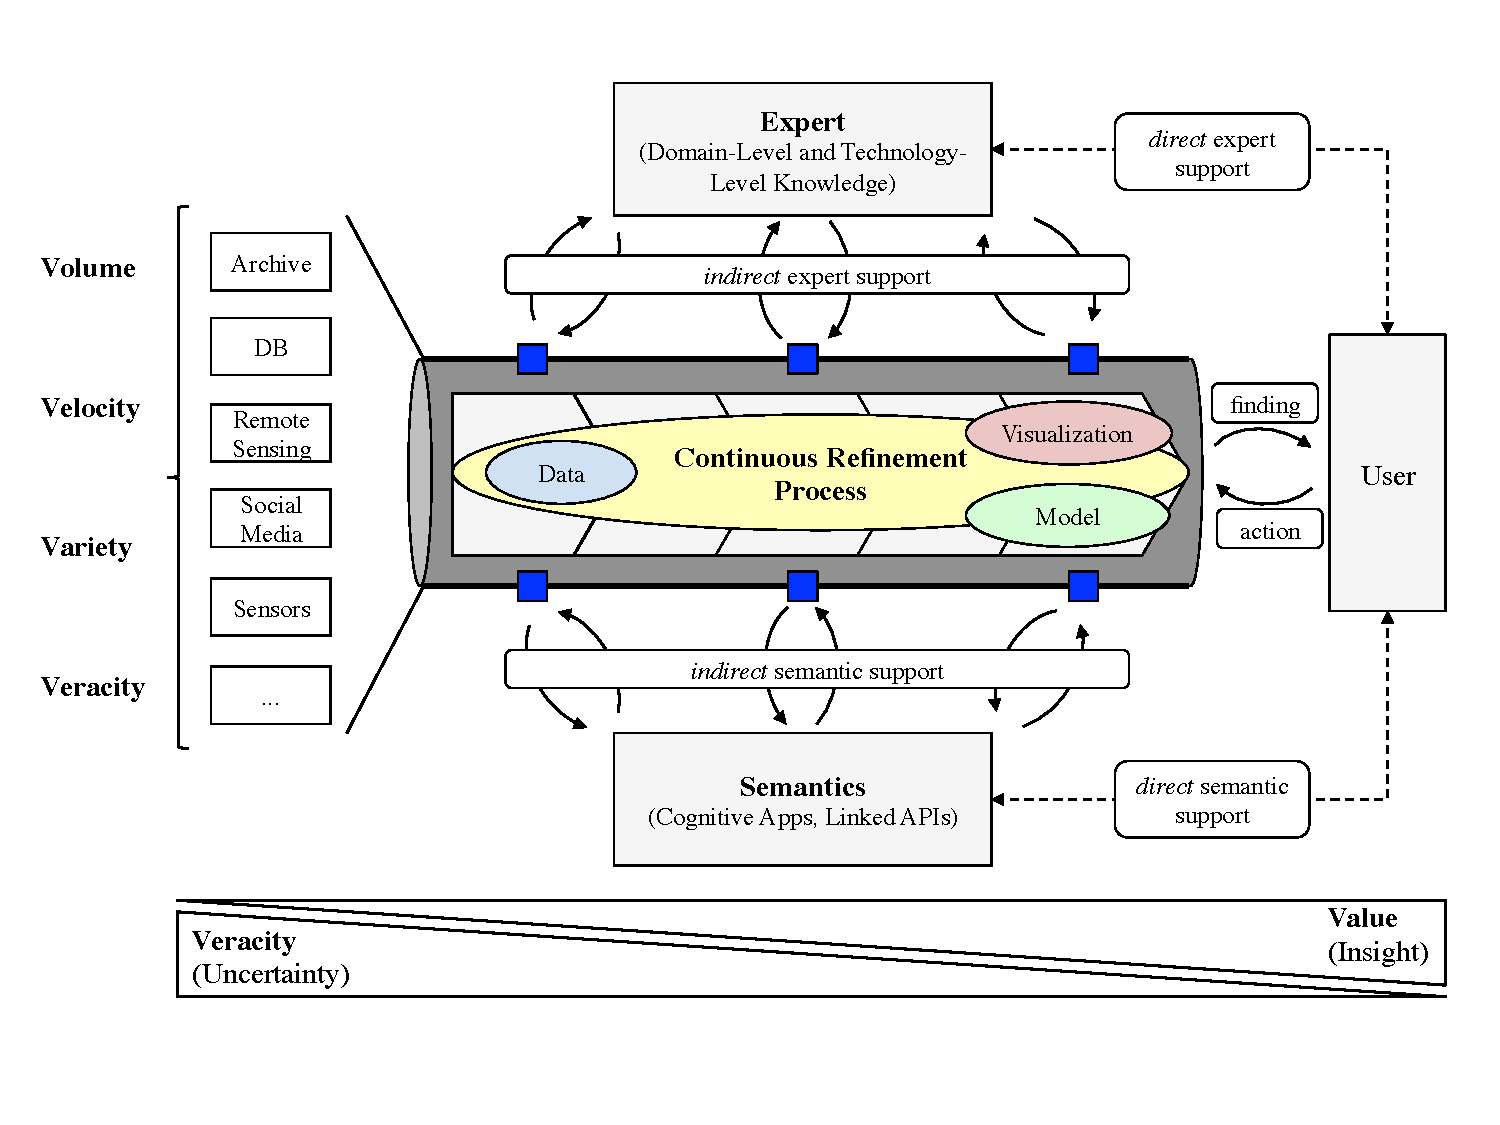
\includegraphics[width=\textwidth]{figures/biggis-workflow}
	\caption{Generic integrated analytical pipeline approach of BigGIS platform showing general purpose Continuous Refinement Process. Overcoming the usability gap between raw data and feature extraction (information gain, insight) and handling uncertainty in acquired data through indirect and direct semantic-level and expert-level support leveraged by the Knowledge Generation Model for Visual Analytics is one main contribution of BigGIS. Indirect support results from defined Refinement Gates (R-Gates \textcolor{blue}{\quadrat}).}
	\label{fig:biggisworkflow}
\end{figure*}

\begin{itemize}
	\item \textcolor{red}{ToDO@Patrick} (1st draft: Describing general aspects of the CRM in BigGIS. Subsubsections should match the contribution/content mentioned in the Introduction's last paragraph).
	\item \textcolor{red}{ToDO@Patrick} (1st draft: High-Level description of end-to-end workflow)
\end{itemize}

\subsubsection{Data}

\subsubsection{Semantic Reasoning}
Locating all available data sources that are relevant for meaningful findings in analytical processes is hard to do when it has to be done manually. Semantic Web technology helps to describe data sources semantically using	widely-used vocabularies. Furthermore, semantic reasoning enables machines to discover suitable sources even if they are described differently, provided that an appropriate ontology supports the system.

\subsubsection{Knowledge Extraction and Generation}

\subsubsection{Integrated Analytical Pipeline}

\subsubsection{Dealing with Uncertainty}
When considering uncertain data like volunteered geographic information and participatory sensing data in geographical information systems, we also have to deal with uncertainty. To address this challenge, we apply semantic reasoning on the provenance information of data sources in order to infer a level of uncertainty that can be considered in the analytical processes.

\subsection{Challenges}
\label{sec:chls}

\begin{itemize}
	\item \textcolor{red}{ToDO@all}: What challenges do we expect to have? According to the structure of the paper we should use the \texttt{\textbackslash subsubsection} from Section \ref{sec:crm} as orientation
	\item Handling big data related requirements: volume, velocity, variety and veracity
	\item challenge 3
\end{itemize}

\section{Use Cases}
\textcolor{red}{ToDO@all} BigGIS will support decision making in multiple use cases which require processing of large and heterogeneous data sets. The prototype will be evaluated on three scenarios: (1) smart city and health, i.e. predicting urban heat islands, (2) environmental management, i.e. prediciting spread of invasive pests, (3) emergency management, i.e. predicting dispersion of toxic gases.

\textcolor{blue}{Comment: We have to describe why these use-cases can only be tackled in a big data context or why they would profit from the availability of big data. One example with the environmental management scenario, where farmers can provide real-time (velocity) data, in different forms (private weather station (numbers), photos of the spotted-wing drosophila/ambrosia, messages (text) => variety), but it comes with a low veracity/high uncertainty. And the combination of this data with the already available data (volume) we can make predictions possible or make them better than before.} 


\section{Discussion and Future Work}
\textcolor{red}{ToDO@all} (In the discussion part we discuss the advantages and disadvantages of our approach. In the conclusion we again shortly summarize in our own words what we just presented and give insight about future work.)
%\end{document}  % This is where a 'short' article might terminate

%ACKNOWLEDGMENTS are optional
\section{Acknowledgements}
\textcolor{red}{ToDO@all} What to place here?

\textcolor{blue}{This research has been funded by the Federal Ministry of Education and Research of Germany (subsidy program IKT 2020 - Forschung f\"ur Innovation).}

%
% The following two commands are all you need in the
% initial runs of your .tex file to
% produce the bibliography for the citations in your paper.
\bibliographystyle{abbrv}
\bibliography{biggis-paper}  % sigproc.bib is the name of the Bibliography in this case
% You must have a proper ".bib" file
%  and remember to run:
% latex bibtex latex latex
% to resolve all references
%
% ACM needs 'a single self-contained file'!
%
%APPENDICES are optional
%\balancecolumns
%\appendix
%Appendix A


\end{document}
